% Manual_MILP_BH_cyclic_ec_vector_en.txt
% ver1: Jan 12, 2021

\documentclass[11pt, titlepage, dvipdfmx, twoside]{article}
\linespread{1.1}

\usepackage{amsfonts}
\usepackage{amssymb}
\usepackage{amsmath}
\usepackage{amsthm}
\newtheorem{theorem}{Theorem}
\newtheorem{lemma}[theorem]{Lemma}
\usepackage{enumitem}
\usepackage{geometry}
\geometry{left=2.5cm, right=2.5cm, top=2.5cm, bottom=2.5cm}

\usepackage{mathtools}
\usepackage{comment}
\usepackage[dvipdfmx]{graphicx}
\usepackage{float}
\usepackage{framed}
\usepackage{graphicx}
\usepackage{subcaption}
\usepackage{listings}
\usepackage{color}
\usepackage{url}
 
\definecolor{codegreen}{rgb}{0, 0.6, 0}
\definecolor{codegray}{rgb}{0.5, 0.5, 0.5}
\definecolor{codepurple}{rgb}{0.58, 0, 0.82}
\definecolor{backcolour}{rgb}{0.95, 0.95, 0.92}

\newcommand{\tname}{6Hc} 
%%  target name used for the example 

\newcommand{\dist}{\mathrm{dist}}

\title{\Huge{Inferring a 2-Lean Cyclic Chemical Graph with Bounded Branch-Height
			  from a Trained ANN using MILP}}

\begin{document}

% The following makeatletter must be after begin{document}
\makeatletter 
\let\c@lstlisting\c@figure
\makeatother

\date{\today}

\maketitle

% \cleardoublepage

\thispagestyle{empty}
\tableofcontents
\clearpage

\pagenumbering{arabic}


\section{Outline}
\label{sec:Intro}

This note explains how to use an implementation of a mixed-integer
linear programming (MILP) formulation that can infer
a vector of graph descriptors given a target value and the 
weights and bias values of a trained artificial neural network (ANN).

The MILP is implemented in Python, 
using the PuLP modeling module of the 
COIN-OR package~\cite{PuLP1,PuLP2,PuLP3,PuLP4}.

To begin with, we give a list of the files that accompany this note.

\begin{itemize}

\item Folder {\tt source\_code}\\
A folder containing four python scripts that implement
an MILP formulation for inferring feature vectors
of cyclic chemical graphs from a trained ANN,
and files containing minimum and maximum values
of each descriptor
in the MILP formulation.

\begin{itemize}

\item {\tt ann\_inverter.py}\\
An implementation of an MILP formulation 
for the Inverse problem on  ANNs~\cite{AN19}.

\item {\tt cyclic\_graphs\_MILP\_ec\_id\_vector.py}\\
A python script that contains functions to initialize the variables and prepare 
the constraints for an MILP
formulation for inferring cyclic chemical graphs with 
a prescribed topological structure~\cite{cyclic_BH_arxiv}.

\item {\tt infer\_cyclic\_graphs\_ec\_id\_vector.py}\\
A python script that prepares the data and executes 
the MILP formulation for given input data.
Further details on the use of this script
are given in Section~\ref{sec:Exp}.

\item {\tt read\_instance\_BH\_cyclic\_v05.py}\\
A python script that contains necessary functions
to read the topological specification from a given textual file.

\item Folder {\tt topological\_description}\\
A folder containing six textual files each giving a chemical specification as detailed 
in~\cite{cyclic_BH_arxiv}.
%
\begin{itemize}
 \item {\tt instance\_a.txt} 
 \item {\tt instance\_b1.txt} 
 \item {\tt instance\_b2.txt} 
 \item {\tt instance\_b3.txt}
 \item {\tt instance\_b4.txt}  
 \item {\tt instance\_c.txt} 
 \item {\tt instance\_d.txt} 
\end{itemize}

\item Folder {\tt ANN}\\
A folder containing information on trained artificial neural networks (ANNs) for three target properties:
Flash point (closed cup) (Fp), Lipophylicity (Lp), and Solubility (Sl).
For each of the above three properties, ${\tt property} \in \{{\tt FP, LP, SL}\}$ three files are provided:
%
\begin{itemize}
\item {\tt property\_desc.csv}\\
A comma-separated value file containing descriptors
used in the training of the ANN.

\item {\tt property\_biases.txt}\\
A file containing the values of the biases of a trained ANN.

\item {\tt property\_weights.txt}\\
A file containing the values of the weights of a trained ANN.
\end{itemize}
%
For each of the files, the data format is explained in Section~\ref{sec:InOut},
and an actual example is given in Section~\ref{sec:Exp}.

\item {\tt fv4\_cyclic\_stdout.cpp}\\
A C++ program that calculates the feature vector of 
a chemical graph stored in SDF format.
The input and output of this program are customized to work with 
the python script {\tt infer\_cyclic\_graphs\_ec\_id\_vector.py}
in order to verify the descriptor values
of the graph inferred as a solution to the MILP (if one exists).
This source file should be compiled into an executable file
with the name {\tt fv}.

\item {\tt fv}\\
An executable binary file of the above C++ program.
This executable has been compiled 
by {\tt gcc} version 5.4.0
on a PC running the Linux Mint 18.3 operating system.
%
\end{itemize}
\end{itemize}



The remaining of this note is organized as follows.
Section~\ref{sec:Pre} gives an explanation 
of the used terms and notation.
%
Section~\ref{sec:InOut} explains the 
input and output data of the program,
and Sec.~\ref{sec:Exp} gives a concrete
example of input data and the results form the computation.

% \newpage

\section{Terms and Notation}
\label{sec:Pre}
%
This section explains the terms and notation used in this note.


\begin{itemize}

\item {\bf Feature vector}\\
%
A {\em feature vector} stores numerical values of certain parameters,
called {\em descriptors}.
In this work, we choose graph-theoretical descriptors, such as number of 
non-hydrogen atoms, number of vertices of certain degree, etc.

\item {\bf Artificial neural network - ANN}\\
%
Artificial neural networks are one of the methods in machine learning.
They provide a means to construct a correlation function between 
pairs of feature vectors as input and target data as output.


\item {\bf Input, hidden, and output layer}\\
%
We deal with the multilayer perceptron model 
of feed-forward neural networks.
These neural networks are constructed of several {\em layers}.
First comes the \emph{input layer}, where each neuron takes as input
one value of the feature vector.
Next come the \emph{hidden layers}, where the 
values from the input layer are propagated in a feed-forward manner,
such that each node in one layer is connected to all the nodes of the next layer. 
Finally, the output is delivered at the \emph{output layer}.
We deal with predicting the value of a single target,
and hence we assume that the output layer comprises a single node.

\item {\bf Weights}\\
%
Each edge connecting two nodes in an ANN is assigned a real value,
called a \emph{weight}.
Part of the \emph{learning} process of ANNs is to determine values for each of the weights
based on known pairs of feature vectors and target values.

\item {\bf Biases}\\
Each node of an ANN except for the nodes in the input layer
is assigned a real value, called a {\em bias},
which, just like the edge weights, is determined through the learning process.


\item {\bf Activation function}\\
%
In an ANN, each node produces an output as a function, called the \emph{activation function}, 
of its input.
We assume that each node has the Rectified Linear-Unit (ReLU) function 
as its activation function,
which can be expressed exactly in the MILP formulation
for the inverse problem on ANNs~\cite{AN19}.
%https://scikit-learn.org/stable/modules/generated/sklearn.neural\_network.MLPRegressor.html

\item {\bf Mixed-Integer Linear Programming (MILP)}\\
%
A type of a mathematical programming problem
where all the constraints are given as linear expressions, and
some of the decision variables are required to take
only integer values.
For more details, see any standard reference, e. g.~\cite{LP}.


\item {\bf Graph} \\
An abstract combinatorial construction comprising
a finite set of {\em vertices}, and a finite set of {\em edges},
where each edge is a pair of vertices.
We treat {\em undirected} graphs,
i. e., graphs where edges are unordered pairs of vertices.
For more information, see e. g.~\cite{graph}.

\end{itemize}

% \newpage

\section{The Program's Input and Output}
\label{sec:InOut}

This section explains the format of the input and the output of the program.
Section~\ref{sec:section3_1} illustrates an example of the program's input format,
and Section~\ref{sec:section3_2} gives a concrete computational example.
Following, Section~\ref{sec:section3_3} illustrates an example of the program's output format,
and Section~\ref{sec:section3_4} gives a concrete computational example.


\subsection{Program Input}
\label{sec:section3_1}

This section gives an explanation of the input to the program.

First
the input requires three textual files containing \\
~~~~- the descriptor names, in csv format \\
~~~~- the weights and biases of a trained ANN in textual format.\\
For a common prefix {\tt TT} which the program accepts as a command-line parameter,
these files must be saved with file names {\tt TT\_desc.csv}, 
{\tt TT\_weights.txt} and {\tt TT\_biases.txt} for the files containing
the descriptor names, the weights, and the biases of a trained ANN, respectively.
%
Next, comes the target value for which we wish to infer 
a chemical graph based on the trained ANN given above.
Following is a chemical specification given in a textual file,
as described in~\cite{cyclic_BH_arxiv}, 
as well as a filename prefix for the output files,  which are described in Sec.~\ref{sec:section3_4}

Finally, comes a choice of MILP solver program to be used.
We can choose \\
~~~~- 1: CPLEX, a commercial MILP solver~\cite{cplex}. \\
(Note, in this case the parameter {\tt CPLEX\_PATH} in the file {\tt infer\_cyclic\_graphs\_ec\_id\_vector.py}
must be set to the correct path of the CPLEX program executable file.) \\
~~~~- 2: CBC, a free and open-source MILP solver. Comes together with the PuLP package for python~\cite{PuLP1}.




\subsection{Input Data Format}
\label{sec:section3_2}

This section presents an actual example of an input instance of the program.
In particular, we give a concrete example of the three input files
mentioned in Section~\ref{sec:section3_1}.

The purpose of this program is to calculate a feature vector that will produce a desired output from a 
given trained ANN.
Figure~\ref{fig:sample} gives an example of a trained ANN.


\begin{figure}[H]
  \centering
  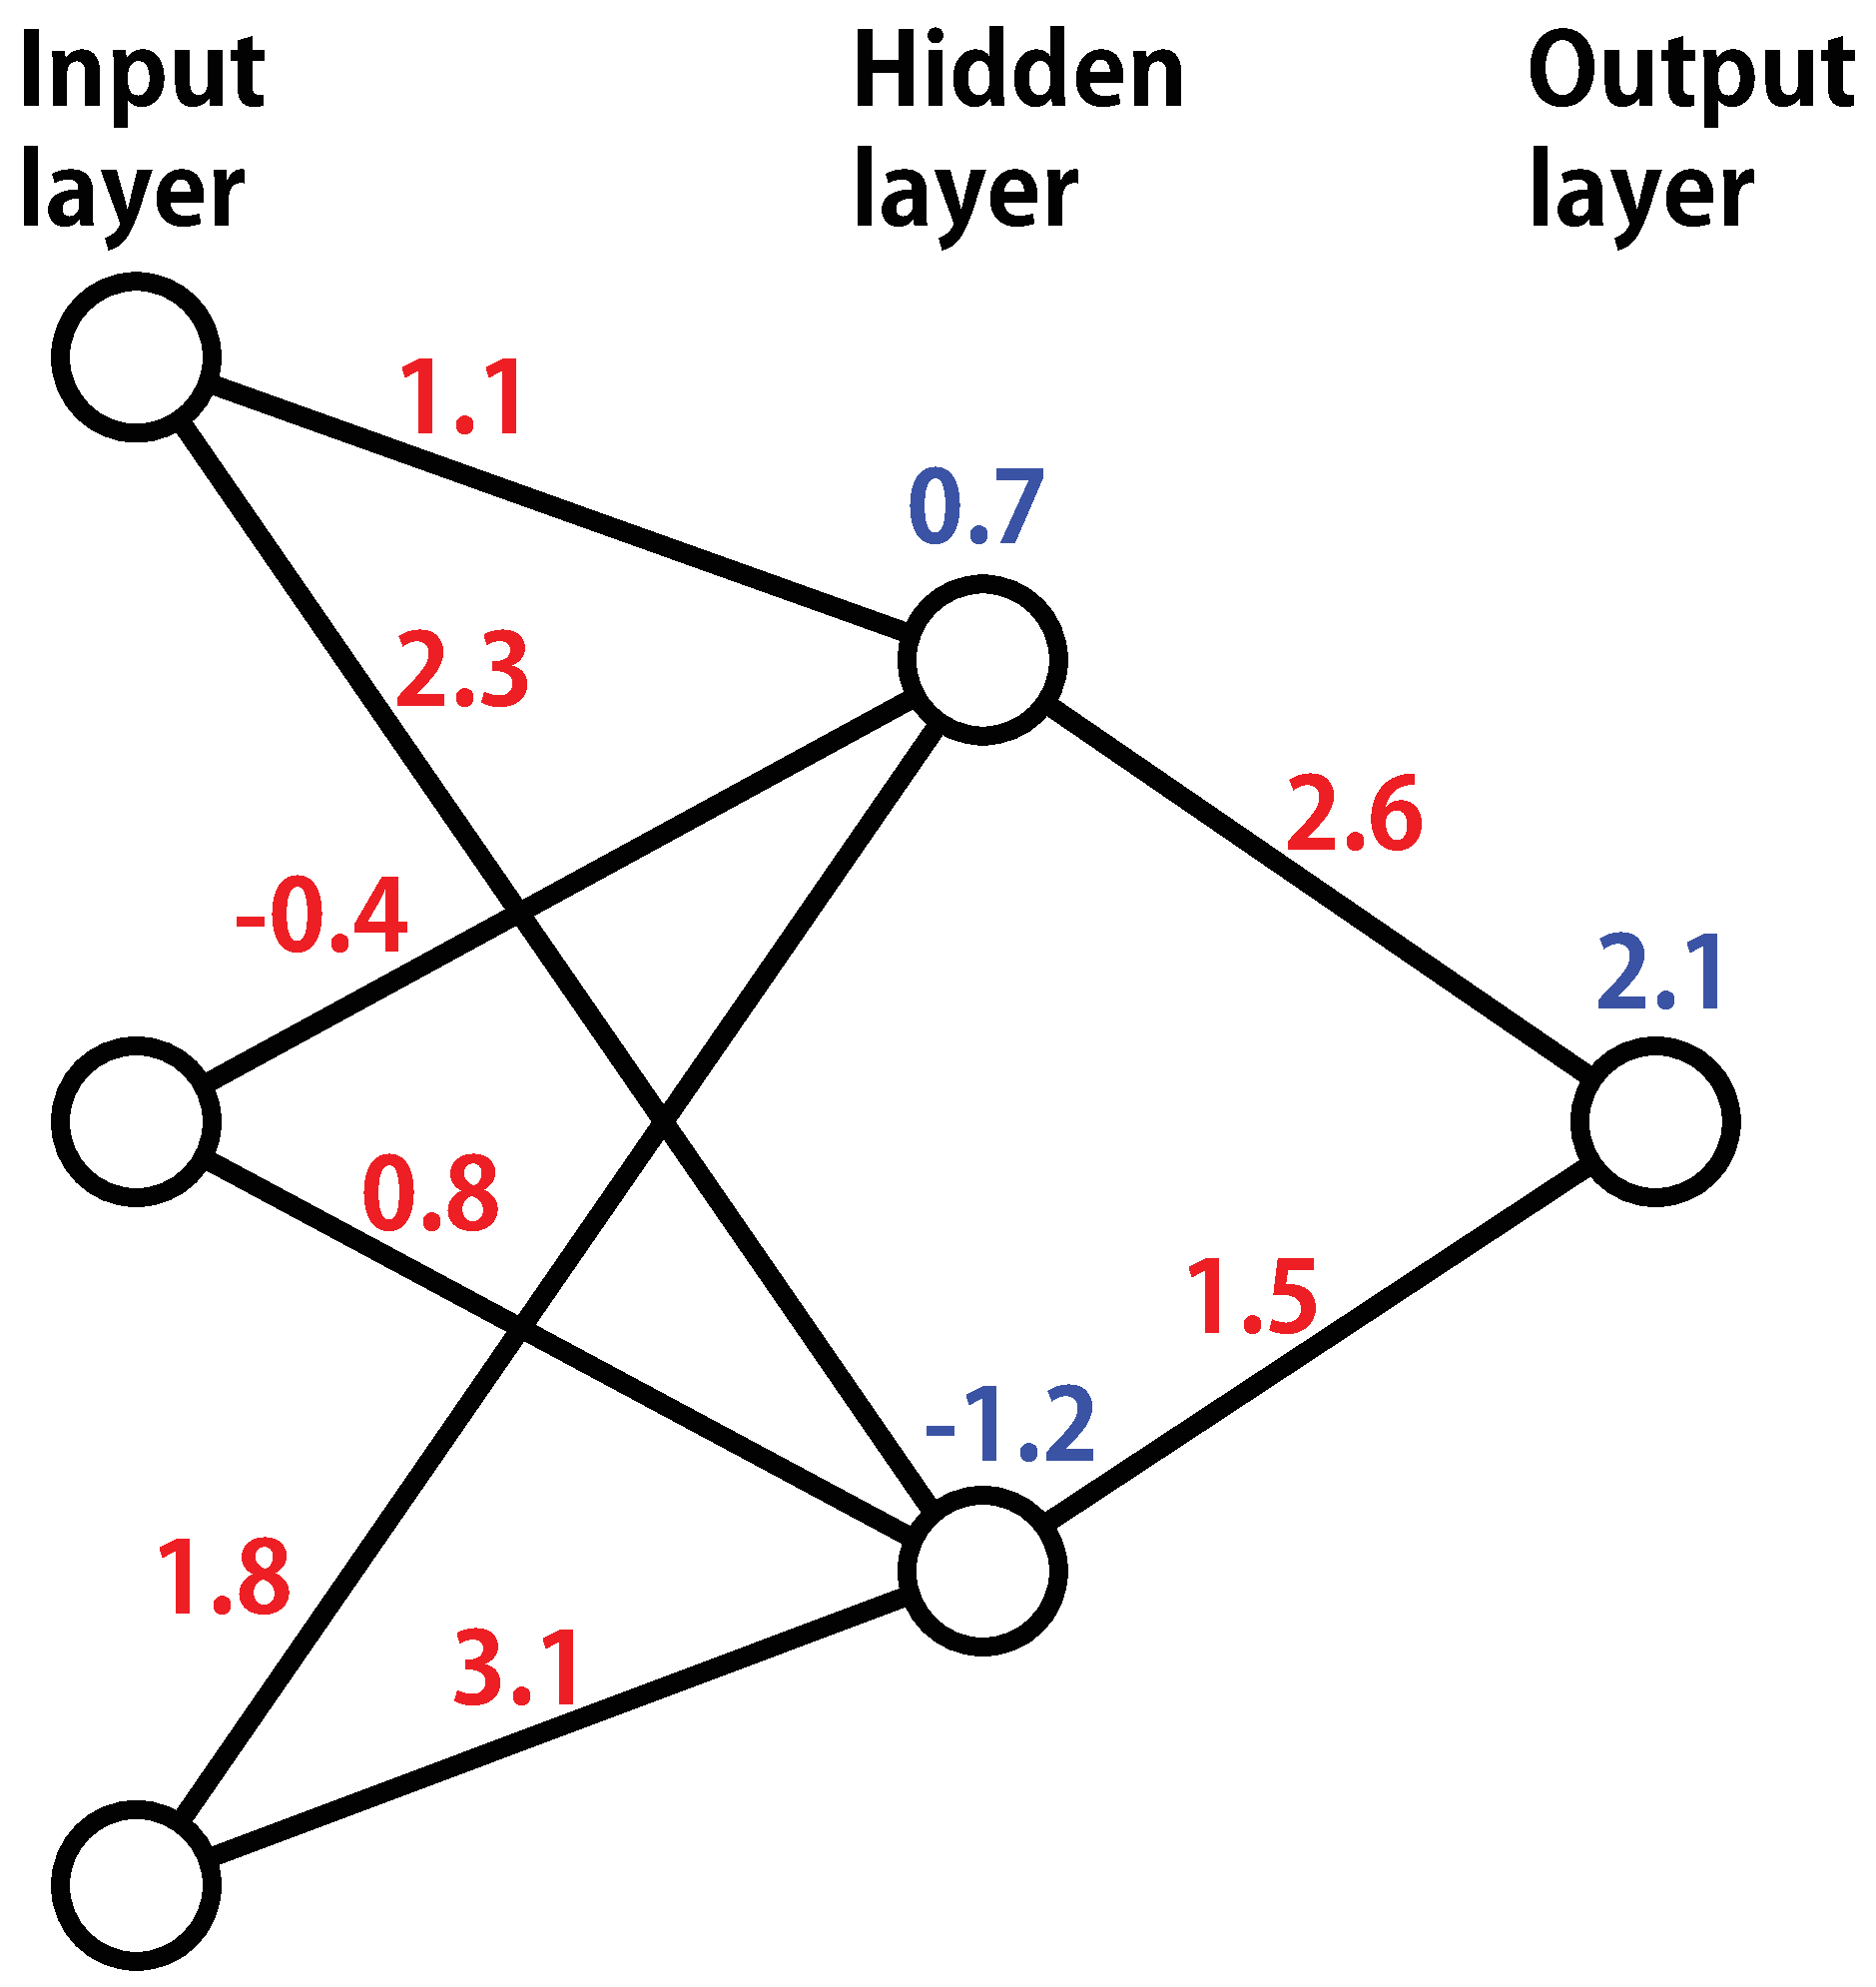
\includegraphics[width=0.5\textwidth]{./fig/ANN_sample_en}
  \caption{An example of a trained ANN.
		      The ANN's weights are given in red numbers, and
		      its biases in blue.
		    }
  \label{fig:sample}
\end{figure}


The information on the trained ANN is written in two text files, containing the information
on the ANN's weights and biases, respectively.
First, we give the structure of the file that contains the information on the ANN's weights.
The first line of this text file contains the information on the ANN's architecture, i. e., 
the number of nodes in each of its layers.
From the second row and onward
follows the information on the 
weights in the ANN.
Each row contains the weights of the edges that are incident to one node of the ANN,
first of the nodes in the input layer, and then for the nodes of the hidden layers.
Following is a textual example for the ANN given in Fig.~\ref{fig:sample}.

\bigskip

\begin{oframed}
{\bf Organization of the text file containing weight data}\\\\
%\bigskip\bigskip
3 2 1\\
1.1 2.3\\
-0.4 0.8\\
1.8 3.1\\
2.6\\
1.5\\
\end{oframed}

\bigskip


Next, comes the text file with the information on the ANN's biases.
The bias values from Fig.~\ref{fig:sample} are given below.

\bigskip

\begin{oframed}
{\bf Bias values}\\\\
%\bigskip\bigskip
0.7\\
-1.2\\
2.1\\
\end{oframed}

\bigskip

Last comes a text file containing data on the feature vector.
The first line of this file contains the names of the descriptors used in the feature vectors.
Following form the second row onward, are the numerical values of the descriptors for each chemical graph
in the training dataset, one row per chemical graph.
For an example, please check one of the files  {\tt TT\_desc.csv},  in the folder {\tt ANN},
where ${\tt property} \in \{{\tt FP, LP, SL}\}$.



\subsection{Program Output}
\label{sec:section3_3}

This section gives an explanation of the output of the program.
If there exists an acyclic chemical graph with a feature vector that
would result with the given target value as a prediction of
the given trained ANN, the program will output the feature vector.
In case such a chemical graph does not exist, the program will report this.
The next section gives an explanation of the output of the program.


\subsection{Output Data Format}
\label{sec:section3_4}

This section describes the output data of the program as
obtained on a personal computer.

Once invoked, the program will print some messages to the standard error
stream, which appear on the terminal.
Once the MILP solver completes the computation,
the status of the computation is printed on the terminal.

\bigskip

\begin{oframed}
{\bf Text output on the terminal}\\\\
%\bigskip\bigskip
\begin{tabular}{l l}
 Initializing Time: 0.809                &         \# Written to {\tt stderr} \\
Start Solving Using CPLEX...      &       \# Written to {\tt stderr} \\
Status: Feasible 				&       \# Solution status \\
MILP y*: 197.922 				&      \# Calculated target value in the MILP  \\
ANN propagated y*: 197.922     &      \# Target value calculated by the trained ANN  \\
All descriptors match    		&      \# Descriptor values due to the MILP and the inferred  graph \\
Solving Time: 16.711                     &      \# Time taken by the MILP solver \\
\end{tabular}



\end{oframed}

Finally, if there exists a feasible solution the program writes to disk two text files.
Recall that as a part of the input the program requires a filename
used for the output files. 
Assume that the supplied parameter is {\tt filename}.
Then, the resulting two text files are named \\
- {\tt filename.sdf} \\
- {\tt filename\_partition.sdf}. 

\noindent
The file {\tt filename.sdf} contains information
on the inferred chemical graph in the SDF (Structure Data File)
format.
For more information see the official documentation (in English) \\
\url{http://help.accelrysonline.com/ulm/onelab/1.0/content/ulm_pdfs/direct/reference/}\\
\phantom{\url{http://}} \url{ctfileformats2016.pdf} \\
for detail.

\noindent
The file {\tt filename\_partition.sdf} contains a 
decomposition of the cyclic graph from the 
file {\tt filename.sdf} into acyclic subgraphs,
as described in~\cite{cyclic_BH_arxiv}.



\section{Invoking the Program and a Computational Example}
\label{sec:Exp}

This section explains how to invoke the program
and explains a concrete computational example.
Following is an example of invoking the
program {\tt infer\_cyclic\_graphs\_ec\_id\_vector.py}.

 


\subsection{Executing the Program}
\label{sec:Exp_1}

First make sure that the terminal is 
correctly directed to the location
of the {\tt source\_code} folder, as described in Sec.~\ref{sec:Intro}. \\

\noindent
{\tt 
 python  infer\_cyclic\_graphs\_ec\_id\_vector.py 
trained\_ann\_filename\_prefix
target\_value \\
 \phantom{python } 
 chemical\_specification
output\_file\_name
solver\_type
 }\\


As an example we use the target property Flash Point (closed cup), 
that is, the files from the trained ANN with filename prefix {\tt FP},
target value 200,
the file {\tt instance\_a.txt} for a chemical specification,
and CPLEX~\cite{cplex} as an MILP solver (parameter value 1).

{\tt 
 python infer\_cyclic\_graphs\_ec\_id\_vector.py 
ANN/FP
200 \\
 \phantom{python } 
chemical\_specification/instance\_a.txt
result
1
 }\\


By executing the above command, the following text should appear on the terminal prompt.

\bigskip

\begin{oframed}
{\bf Text output on the terminal}\\\\
%\bigskip\bigskip
 Initializing Time: 0.809  \\
Start Solving Using CPLEX...\\
Status: Feasible 		\\
MILP y*: 197.922 		\\
ANN propagated y*: 197.922 \\
All descriptors match    	\\
Solving Time: 16.711       
\end{oframed}

The contents of the output files {\tt result.sdf} and
{\tt result\_partition.txt} are as follows.

\bigskip

\begin{oframed}
{\bf File {\tt result.sdf}}\\\\
\begin{verbatim}
 1
MILP_cyclic
ec_id_vector
 43 46  0  0  0  0  0  0  0  0999 V2000 
    0.0000    0.0000    0.0000 C   0  0  0  0  0  0  0  0  0  0  0  0
    0.0000    0.0000    0.0000 C   0  0  0  0  0  0  0  0  0  0  0  0
    0.0000    0.0000    0.0000 C   0  0  0  0  0  0  0  0  0  0  0  0
    0.0000    0.0000    0.0000 C   0  0  0  0  0  0  0  0  0  0  0  0
    0.0000    0.0000    0.0000 C   0  0  0  0  0  0  0  0  0  0  0  0
    0.0000    0.0000    0.0000 O   0  0  0  0  0  0  0  0  0  0  0  0
    0.0000    0.0000    0.0000 C   0  0  0  0  0  0  0  0  0  0  0  0
    0.0000    0.0000    0.0000 C   0  0  0  0  0  0  0  0  0  0  0  0
    0.0000    0.0000    0.0000 N   0  0  0  0  0  0  0  0  0  0  0  0
    0.0000    0.0000    0.0000 C   0  0  0  0  0  0  0  0  0  0  0  0
    0.0000    0.0000    0.0000 C   0  0  0  0  0  0  0  0  0  0  0  0
    0.0000    0.0000    0.0000 C   0  0  0  0  0  0  0  0  0  0  0  0
    0.0000    0.0000    0.0000 C   0  0  0  0  0  0  0  0  0  0  0  0
    0.0000    0.0000    0.0000 N   0  0  0  0  0  0  0  0  0  0  0  0
    0.0000    0.0000    0.0000 C   0  0  0  0  0  0  0  0  0  0  0  0
    0.0000    0.0000    0.0000 C   0  0  0  0  0  0  0  0  0  0  0  0
    0.0000    0.0000    0.0000 C   0  0  0  0  0  0  0  0  0  0  0  0
    0.0000    0.0000    0.0000 C   0  0  0  0  0  0  0  0  0  0  0  0
    0.0000    0.0000    0.0000 C   0  0  0  0  0  0  0  0  0  0  0  0
    0.0000    0.0000    0.0000 C   0  0  0  0  0  0  0  0  0  0  0  0
    0.0000    0.0000    0.0000 C   0  0  0  0  0  0  0  0  0  0  0  0
    0.0000    0.0000    0.0000 C   0  0  0  0  0  0  0  0  0  0  0  0
    0.0000    0.0000    0.0000 C   0  0  0  0  0  0  0  0  0  0  0  0
    0.0000    0.0000    0.0000 C   0  0  0  0  0  0  0  0  0  0  0  0
    0.0000    0.0000    0.0000 C   0  0  0  0  0  0  0  0  0  0  0  0
    0.0000    0.0000    0.0000 C   0  0  0  0  0  0  0  0  0  0  0  0
    0.0000    0.0000    0.0000 C   0  0  0  0  0  0  0  0  0  0  0  0
    0.0000    0.0000    0.0000 C   0  0  0  0  0  0  0  0  0  0  0  0
    0.0000    0.0000    0.0000 C   0  0  0  0  0  0  0  0  0  0  0  0
    0.0000    0.0000    0.0000 N   0  0  0  0  0  0  0  0  0  0  0  0
    0.0000    0.0000    0.0000 C   0  0  0  0  0  0  0  0  0  0  0  0
    0.0000    0.0000    0.0000 C   0  0  0  0  0  0  0  0  0  0  0  0
    0.0000    0.0000    0.0000 C   0  0  0  0  0  0  0  0  0  0  0  0
    0.0000    0.0000    0.0000 O   0  0  0  0  0  0  0  0  0  0  0  0
    0.0000    0.0000    0.0000 C   0  0  0  0  0  0  0  0  0  0  0  0
    0.0000    0.0000    0.0000 C   0  0  0  0  0  0  0  0  0  0  0  0
    0.0000    0.0000    0.0000 C   0  0  0  0  0  0  0  0  0  0  0  0
    0.0000    0.0000    0.0000 O   0  0  0  0  0  0  0  0  0  0  0  0
    0.0000    0.0000    0.0000 C   0  0  0  0  0  0  0  0  0  0  0  0
    0.0000    0.0000    0.0000 C   0  0  0  0  0  0  0  0  0  0  0  0
    0.0000    0.0000    0.0000 O   0  0  0  0  0  0  0  0  0  0  0  0
    0.0000    0.0000    0.0000 C   0  0  0  0  0  0  0  0  0  0  0  0
    0.0000    0.0000    0.0000 C   0  0  0  0  0  0  0  0  0  0  0  0
  1  2  2  0  0  0  0
  1 24  1  0  0  0  0
  2 25  1  0  0  0  0
  2 41  1  0  0  0  0
  3  4  1  0  0  0  0
  3 23  2  0  0  0  0
  3 38  1  0  0  0  0
  4  5  2  0  0  0  0
  4 33  1  0  0  0  0
  5 24  1  0  0  0  0
  6 12  1  0  0  0  0
  6 18  1  0  0  0  0
  7  9  1  0  0  0  0
  7 11  2  0  0  0  0
  7 28  1  0  0  0  0
  8  9  1  0  0  0  0
  8 10  1  0  0  0  0
 10 11  1  0  0  0  0
 11 12  1  0  0  0  0
 12 17  1  0  0  0  0
 13 14  1  0  0  0  0
 13 17  1  0  0  0  0
 13 19  1  0  0  0  0
 14 15  1  0  0  0  0
 14 16  1  0  0  0  0
 17 18  2  0  0  0  0
 18 22  1  0  0  0  0
 19 20  1  0  0  0  0
 19 21  1  0  0  0  0
 19 23  1  0  0  0  0
 22 23  1  0  0  0  0
 24 25  1  0  0  0  0
 25 26  1  0  0  0  0
 25 27  1  0  0  0  0
 28 29  1  0  0  0  0
 28 30  1  0  0  0  0
 30 31  1  0  0  0  0
 30 32  1  0  0  0  0
 33 34  1  0  0  0  0
 34 35  1  0  0  0  0
 35 36  1  0  0  0  0
 35 37  1  0  0  0  0
 38 39  1  0  0  0  0
 39 40  3  0  0  0  0
 41 42  1  0  0  0  0
 42 43  3  0  0  0  0
M  END
$$$$
\end{verbatim}    
\end{oframed}

\bigskip

\begin{oframed}
{\bf File {\tt result\_partition.txt}}\\\\
\begin{verbatim}
12
9
0 1
10
0 0
11
0 0
12
0 0
13
1 3
17
0 0
18
0 1
19
0 1
22
0 0
23
0 1
24
0 2
25
0 4
15
9 7 11
1 3
9 8 10
0 3
10 11
0 0
11 12
0 0
12 6 18
0 1
12 17
0 0
13 17
0 0
13 19
0 0
17 18
0 0
18 22
0 0
19 23
0 0
22 23
0 0
23 3 4 5 24
4 6
24 1 2 25
3 5
24 25
0 2
\end{verbatim}    
\end{oframed}


\begin{thebibliography}{99}
  \bibitem{AN19} 
    T.~Akutsu and H.~Nagamochi.
    A Mixed Integer Linear Programming Formulation to Artificial Neural Networks,
    in Proceedings of the 2019 2nd International Conference on Information Science and Systems,
    pp.~215--220, https://doi.org/10.1145/3322645.3322683.
    
  \bibitem{cyclic_BH_arxiv}
	  T.~Akutsu and H.~Nagamochi.
	  A Novel Method for Inference of Chemical Compounds with Prescribed Topological Substructures Based on Integer Programming.
	  Arxiv preprint, arXiv:2010.09203
	  
%   \bibitem{graph} 茨木俊秀,永持仁,石井利昌.グラフ理論ー連結構造とその応用ー.朝倉書店,2010. 
%   
%   \bibitem{LP} 福島雅夫.数理計画入門.朝倉書店,2012. 
  \bibitem{LP} J.~Matousek and B.~G\"{a}rtner.
			      Understanding and Using Linear Programming. Springer, 2007.
			      
  \bibitem{graph} M.~S.~Rahman.
			      Basic Graph Theory. Springer, 2017.
  
  \bibitem{PuLP1} A Python Linear Programming API, \url{https://github.com/coin-or/pulp}.
  
  \bibitem{PuLP2} Optimization with PuLP, \url{http://coin-or.github.io/pulp/}.
  
  \bibitem{PuLP3} The Python Papers Monograph, \url{https://ojs.pythonpapers.org/index.php/tppm/article/view/111}.
  
  \bibitem{PuLP4} Optimization with PuLP, \url{https://pythonhosted.org/PuLP/}.
  
  \bibitem{cplex}
{IBM ILOG CPLEX Optimization Studio~12.8 User Manual}.
\newblock
  \url|https://www.ibm.com/support/knowledgecenter/SSSA5P_12.8.0/ilog.odms.studio.help/pdf/usrcplex.pdf|.
  
\end{thebibliography}

\end{document}
